\chapter{Implementacija i korisničko sučelje}
		
		
		\section{Korištene tehnologije i alati}
		
			Komunikacija u timu je ostvarena korištenjem aplikacije Discord\footnote{\url{https://discord.com/}}. Komunikacija s asistenticom grupe je ostvarena korištenjem aplikacije Microsoft Teams\footnote{\url{https://www.microsoft.com/hr-hr/microsoft-teams/group-chat-software/}} Za izradu UML dijagrama korišten je alat Visual Paradigm Online\footnote{\url{https://online.visual-paradigm.com/}}. Za upravljanje izvornim kodom korišten je alat Git\footnote{\url{https://git-scm.com/}}. Udaljeni repozitorij projekta nalazi se na platformi Gitlab\footnote{\url{https://gitlab.com/}}. Za upravljanje zadacima na projektu korištena je aplikacija Trello\footnote{\url{https://trello.com/}}.
			
			Kao razvojno okruženje na backendu je koršten IntelliJ\footnote{\url{https://www.jetbrains.com/idea/}}, a na frontendu je korišten Visual Studio Code\footnote{\url{https://code.visualstudio.com/}}. Tehnologije korištene za razvoj backenda su radni okvir Spring Boot\footnote{\url{https://spring.io/projects/spring-boot}} i programski jezik Java\footnote{\url{https://www.java.com/en/}}. Tehologije korištene za razvoj frontenda su biblioteka React\footnote{\url{https://reactjs.org/}} i programski jezik JavaScript\footnote{\url{https://www.javascript.com/}}. Za automatizirano testiranje korišten je alat Selenium WebDriver\footnote{\url{https://www.selenium.dev/documentation/webdriver/}} te programski jezici Java i Python\footnote{\url{https://www.python.org/}}. Za puštanje aplikacije u pogon korištena je platforma Heroku\footnote{\url{https://www.heroku.com/}}.
			
			
			\eject 
		
	
		\section{Ispitivanje programskog rješenja}
					
			\subsection{Ispitivanje komponenti}

			Ispitivanje komponenti ostvareno je korištenjem Spring Boot i JUnit alata za ispitivanje.
			U nastavku su opisani provedeni testovi, te su priloženi kodovi.

			Testovi 1-4 testiraju Account kontroler.
			Inicijalizacijska metoda za testove 1-4 izgleda ovako:

			\begin{lstlisting}[language=Java, breaklines=true]
    @BeforeEach
    public void init() {
        Street street = new Street(1L, "Testna ulica", 1, 5);
        street.setDistrict(new District(1L, "Testni kvart"));
        home = new Home(1L, 1L, street);

        account = new Account(1L, "John", "Doe", "johndoe@gmail.com", "pass123",
                home, null, false);
        account.setRoles(new ArrayList<>());
    }
			\end{lstlisting}

			Testovi 5 i 6 testiraju Post kontroler.
			Inicijalizacijska metoda za testove 5 i 6 izgleda ovako:

			\begin{lstlisting}[language=Java, breaklines=true]
    @BeforeEach
    public void init() {
        District district = new District(1L, "Testni kvart");
        Street street = new Street(1L, "Testna ulica", 1, 5);
        street.setDistrict(district);
        home = new Home(1L, 1L, street);

        account = new Account(1L, "John", "Doe", "johndoe@gmail.com", "pass123",
                home, null, false);

        postThread = new PostThread(1L, "Example", new ArrayList<>(), null, district);

        post = new Post(1L, "First post",
                null,
                null, postThread, account);

        post.setThreadId(postThread.getId());
    }
			\end{lstlisting}

			U prvom ispitnom slučaju ispitan je pokušaj dobavljanja liste svih korisničkih računa.
			Očekivani rezultat je uspješno dobavljanje liste u JSON obliku te HTTP status 200 (OK).

			\begin{lstlisting}[language=Java, breaklines=true]
    @Test
    public void givenAccountsList_whenGetAccountsList_ThenReturnJsonArray() throws Exception {
        List<Account> accounts = Collections.singletonList(account);

        given(accountService.listAll()).willReturn(accounts);

        mvc.perform(get("/accounts")
                .contentType(MediaType.APPLICATION_JSON).accept(MediaType.APPLICATION_JSON))
                .andExpect(status().isOk())
                .andExpect(jsonPath("$", hasSize(1)))
                .andExpect(jsonPath("$[0].firstName").value("John"));
    }
			\end{lstlisting}

			U drugom ispitnom slučaju testiran je rubni slučaj u kojem ne postoji niti jedan korisnički račun, a lista
			korisničkih računa se pokušava dohvatiti. Očekivani rezultat je uspješno dobavljanje prazne liste u JSON obliku te HTTP status 200 (OK).

			\begin{lstlisting}[language=Java, breaklines=true]
	@Test
    public void givenEmptyAccountsList_whenGetAccountsList_thenReturnEmptyJsonArray() throws Exception {
        List<Account> accounts = Collections.emptyList();

        given(accountService.listAll()).willReturn(accounts);

        mvc.perform(get("/accounts")
                .contentType(MediaType.APPLICATION_JSON).accept(MediaType.APPLICATION_JSON))
                .andExpect(status().isOk())
                .andExpect(jsonPath("$", empty()));
    }
			\end{lstlisting}

			U trećem ispitnom slučaju ispitan je pokušaj izrade novog korisničkog računa, dok je pritom priložena email adresa koju neki postojeći korisnik već koristi. Očekivani rezultat je neuspješna izrada korisničkog računa te HTTP status 400 (Bad Request).

			\begin{lstlisting}[language=Java, breaklines=true]
    @Test
    public void givenEmailList_whenCreateAccountWithExistingEmail_thenCauseError400() throws Exception {
        given(accountService.getEmailsFromAccounts()).willReturn(Collections.singletonList("johndoe@gmail.com"));

        mvc.perform(post("/accounts")
                .content(new ObjectMapper()
                        .writeValueAsString(new Account("Johnny", "Doe",
                                "johndoe@gmail.com", "pass123", home, null,
                                false)
                        )
                ).contentType(MediaType.APPLICATION_JSON).accept(MediaType.APPLICATION_JSON)
        ).andExpect(status().isBadRequest());
    }
			\end{lstlisting}

			U četvrtom ispitnom slučaju ispitan je pokušaj dodjele uloge "Stanovnik" postojećem korisniku preko "/accounts/grantRole/" endpointa.
			Očekivani rezultat je uspješna dodjela uloge "Stanovnik" korisniku te HTTP status 200 (OK).

			\begin{lstlisting}[language=Java, breaklines=true]
    @Test
    public void whenGrantRole_thenReturnRole() throws Exception {
        given(accountService.fetch(any(Long.class))).willReturn(account);
        given(accountService.existsById(eq(1L))).willReturn(true);
        given(roleService.findByName(any(String.class))).willReturn(java.util.Optional.of(new Role("Stanovnik")));

        mvc.perform(put("/accounts/grantRole/{id}",1)
                .content("Stanovnik").contentType(MediaType.APPLICATION_JSON).accept(MediaType.APPLICATION_JSON)
        ).andExpect(status().isOk())
                .andExpect(jsonPath("$.name").value("Stanovnik"));
    }
			\end{lstlisting}

			U petom ispitnom slučaju ispitan je pokušaj izrade nove objave uz priložen tekst objave i priložen id postojeće dretve. Očekivani rezultat je uspješna izrada nove objave koja sadrži priložen tekst, te HTTP status 201 (Created).

			\begin{lstlisting}[language=Java, breaklines=true]
    @Test
    public void givenPost_whenCreatePost_thenReturnPostAsJson() throws Exception {
        Post post2 = new Post(2L, "Second post",
                null,
                null, postThread, account);

        post2.setThreadId(postThread.getId());
        given(accountService.fetch(any(Long.class))).willReturn(account);
        given(postService.createPost(any(Post.class), eq(postThread.getId()))).willReturn(post2);
        given(postService.existsById(eq(post2.getId()))).willReturn(false);
        given(postThreadService.existsById(eq(postThread.getId()))).willReturn(true);

        mvc.perform(post("/posts/{id}",1)
                .content(new ObjectMapper().writeValueAsString(post2))
                .contentType(MediaType.APPLICATION_JSON).accept(MediaType.APPLICATION_JSON))
                .andExpect(status().isCreated())
                .andExpect(jsonPath("$.id").value(2))
                .andExpect(jsonPath("$.content").value("Second post"));
    }
			\end{lstlisting}

			U šestom ispitnom slučaju ispitan je pokušaj dohvaćanja objave preko nepostojećeg id-a.
			Očekivani rezultat je neuspješno dohvaćanje objave te HTTP status 400 (Bad Request).

			\begin{lstlisting}[language=Java, breaklines=true]
    @Test
    public void givenNonexistentPostId_whenGetPost_thenCauseError400() throws Exception {
        given(postService.existsById(any(Long.class))).willReturn(false);

        mvc.perform(get("/posts/{id}",5)
                .contentType(MediaType.APPLICATION_JSON)
                .accept(MediaType.APPLICATION_JSON)
        ).andExpect(status().isBadRequest());
    }
			\end{lstlisting}

			Na slici 5.1 je prikazana je snimka zaslona terminala u IntelliJ IDE-u, kao rezultat izvođenja prethodno navedenih šest ispitnih slučajeva.

			\begin{figure}[H]
					\centering
					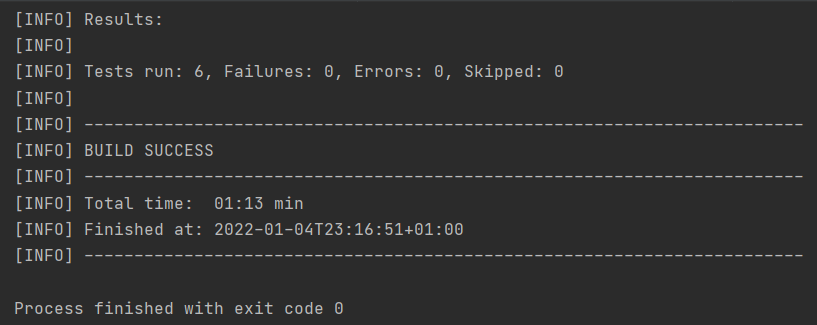
\includegraphics[width=\textwidth,keepaspectratio]{19 ispitivanje komponenti.png}
					\caption{Rezultati ispitivanja pomoću Spring-a i JUnit-a}
				\end{figure}
			\eject

			\subsection{Ispitivanje sustava}

			Ispitivanje sustava ostvareno je korištenjem Selenium WebDrivera i programskog jezika Python. U nastavku su opisani provedeni testovi, te su priloženi kodovi.

			U prvom ispitnom slučaju ispitan je pokušaj prijave s emailom koji nije povezan niti jedan račun, tj. emailom koji ne postoji u sustavu. Očekivani izlaz je neuspjeh pri pokušaju prijave.

			\begin{lstlisting}[language=Python, breaklines=true]
def test1() -> bool:
    driver = webdriver.Firefox()
    driver.get("http://localhost:3000/login")
    driver.find_element_by_name("username").send_keys("stanovnik@stanovnik.com")
    driver.find_element_by_name("password").send_keys("stanovnik")
    driver.find_element_by_css_selector("button[type='submit']").click()
    try:
        driver.find_element_by_class_name("logout")
    except NoSuchElementException:
        driver.close()
        return True
    driver.close()
    return False
			\end{lstlisting}

			U drugom ispitnom slučaju ispitan je pokušaj registracije s neispravnim podacima, konkretno s emailom koji je zadan u krivom formatu. Očekivani izlaz je neuspjeh pri pokušaju registracije.

			\begin{lstlisting}[language=Python, breaklines=true]
def test2() -> bool:
    driver = webdriver.Firefox()
    driver.get("http://localhost:3000/login")
    driver.find_element_by_css_selector("button[type='button']").click()
    driver.find_element_by_name("firstname").send_keys("Stanovnik")
    driver.find_element_by_name("lastname").send_keys("Stanovnikic")
    driver.find_element_by_name("username").send_keys("stanovnik")
    driver.find_element_by_name("password").send_keys("stanovnik")
    dropdown = driver.find_element_by_class_name("css-tlfecz-indicatorContainer")
    dropdown.click()
    actions = ActionChains(driver)
    actions.move_to_element(dropdown).send_keys("Ulica 1 Kvarta 1").key_down(Keys.ENTER).key_up(Keys.ENTER).perform()
    driver.find_element_by_name("streetnumber").send_keys("7")
    driver.find_element_by_css_selector("button[type='submit']").click()
    try:
        driver.find_element_by_class_name("logout")
    except NoSuchElementException:
        driver.close()
        return True
    driver.close()
    return False
			\end{lstlisting}

			U trećem ispitnom slučaju ispitan je pokušaj registracije gdje su svi uneseni podaci valjani. Očekivani izlaz je uspjeh pri pokušaju registracije i preusmjeravanje na početnu stranicu korisnikovog kvarta.

			\begin{lstlisting}[language=Python, breaklines=true]
def test3() -> bool:
    driver = webdriver.Firefox()
    driver.get("http://localhost:3000/login")
    driver.find_element_by_css_selector("button[type='button']").click()
    driver.find_element_by_name("firstname").send_keys("Stanovnik")
    driver.find_element_by_name("lastname").send_keys("Stanovnikic")
    driver.find_element_by_name("username").send_keys("stanovnik@stanovnik.com")
    driver.find_element_by_name("password").send_keys("stanovnik")
    dropdown = driver.find_element_by_class_name("css-tlfecz-indicatorContainer")
    dropdown.click()
    actions = ActionChains(driver)
    actions.move_to_element(dropdown).send_keys("Ulica 1 Kvarta 1").key_down(Keys.ENTER).key_up(Keys.ENTER).perform()
    driver.find_element_by_name("streetnumber").send_keys("7")
    driver.find_element_by_css_selector("button[type='submit']").click()
    try:
        driver.find_element_by_class_name("logout")
    except NoSuchElementException:
        driver.close()
        return False
    driver.close()
    return True
			\end{lstlisting}

			U četvrtom ispitnom slučaju ispitan je pokušaj prijave s emailom za koji postoji korisnički račun, ali s neispravnom lozinkom. Očekivani izlaz je neuspjeh pri pokušaju prijave.

			\begin{lstlisting}[language=Python, breaklines=true]
def test4() -> bool:
    driver = webdriver.Firefox()
    driver.get("http://localhost:3000/login")
    driver.find_element_by_name("username").send_keys("stanovnik@stanovnik.com")
    driver.find_element_by_name("password").send_keys("stanovni")
    driver.find_element_by_css_selector("button[type='submit']").click()
    try:
        driver.find_element_by_class_name("logout")
    except NoSuchElementException:
        driver.close()
        return True
    driver.close()
    return False
			\end{lstlisting}

			U petom ispitnom slučaju ispitan je pokušaj prijave gdje su svi uneseni podaci ispravni. Očekivani izlaz je uspjeh pri pokušaju prijave i preusmjeravanje na početnu stranicu korisnikovog kvarta.

			\begin{lstlisting}[language=Python, breaklines=true]
def test5() -> bool:
    driver = webdriver.Firefox()
    driver.get("http://localhost:3000/login")
    driver.find_element_by_name("username").send_keys("stanovnik@stanovnik.com")
    driver.find_element_by_name("password").send_keys("stanovnik")
    driver.find_element_by_css_selector("button[type='submit']").click()
    try:
        driver.find_element_by_class_name("logout")
    except NoSuchElementException:
        driver.close()
        return False
    driver.close()
    return True
			\end{lstlisting}

			Na slici 5.2 prikazana je snimka zaslona terminala kao rezultat izvođenja prethodno navedenih pet ispitnih slučajeva.

			\begin{figure}[H]
					\centering
					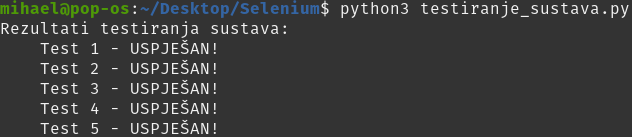
\includegraphics[width=\textwidth,keepaspectratio]{18 ispitivanje sustava.png}
					\caption{Rezultati ispitivanja Selenium WebDriverom}
				\end{figure}
			\eject


		\section{Dijagram razmještaja}

		Na slici 5.3 prikazan je dijagram razmještaja. Sustav je baziran na arhitekturi "klijent-poslužitelj". Korisnici pristupaju aplikaciji korištenjem web preglednika. Na platformi Heroku se nalaze poslužitelji za frontend, backend i bazu podataka. Komunikacija između korisnika i poslužitelja za frontend, te poslužitelja za frontend i poslužitelja za backend, ostvaruje se korištenjem protokola HTTP.

			\begin{figure}[H]
					\centering
					\includegraphics[width=\textwidth,keepaspectratio]{17 dijagram razmještaja.png}
					\caption{Dijagram razmještaja}
				\end{figure}

			\eject

		\section{Upute za puštanje u pogon}
		
		
		Potrebno je napraviti korisnički račun na Heroku i zatim odabirom opcije "New app" stvoriti dvije aplikacije, jednu za frontend i jednu za backend.
		
		S obzirom da je puštanje u pogon značajno jednostavnije s Githuba nego s Gitlaba, potrebno je neki, npr. osobni Github račun, povezati s Heroku računom i potom klonirati projekt dva puta. U prvom kloniranom projektu je potrebno u root direktorij premjestiti sadržaj poddirektorija IzvorniKod/backend-spring-boot, a ostatak sadržaja projekta obrisati. U drugom je projektu potrebno učiniti istu stvar za sadržaj poddirektorija IzvorniKod/frontend-react. Zatim je u svakom projektu na main grani potrebno odabrati opciju "Deploy to Heroku". 
		
		Na Heroku Vas dočeka stranica poput one na slici 5.4. Kada ste u pogon pustili frontend i backend, potrebno je u datoteku .env.production na frontend projektu napisati točan URL na kojem se nalazi backend. Primjer je pokazan na slici 5.5.

		Konačni je korak napuniti bazu s nekom .sql skriptom. Pri puštanju u pogon backenda, automatski se stvori i baza podataka. Na slici 5.4 vidljiva je poveznica "Resources". Potrebno je odabrati ju, zatim je potrebno pod "add-ons" odabrati "heroku postgres" i dočekaju Vas podaci slični onima na slici 5.6. Zatim je potrebno otvoriti pgAdmin, i odabrati opciju "Create Server", kao što je prikazano na slici 5.7. Dalje je potrebno slijediti upute i unijeti podatke poput onih na slici 5.6, i konačno, kada je baza podataka povezana lokalno s pgAdminom, potrebno je odabirom na "Query tool" unijeti željenu .sql skriptu.
		
				\begin{figure}[H]
					\centering
					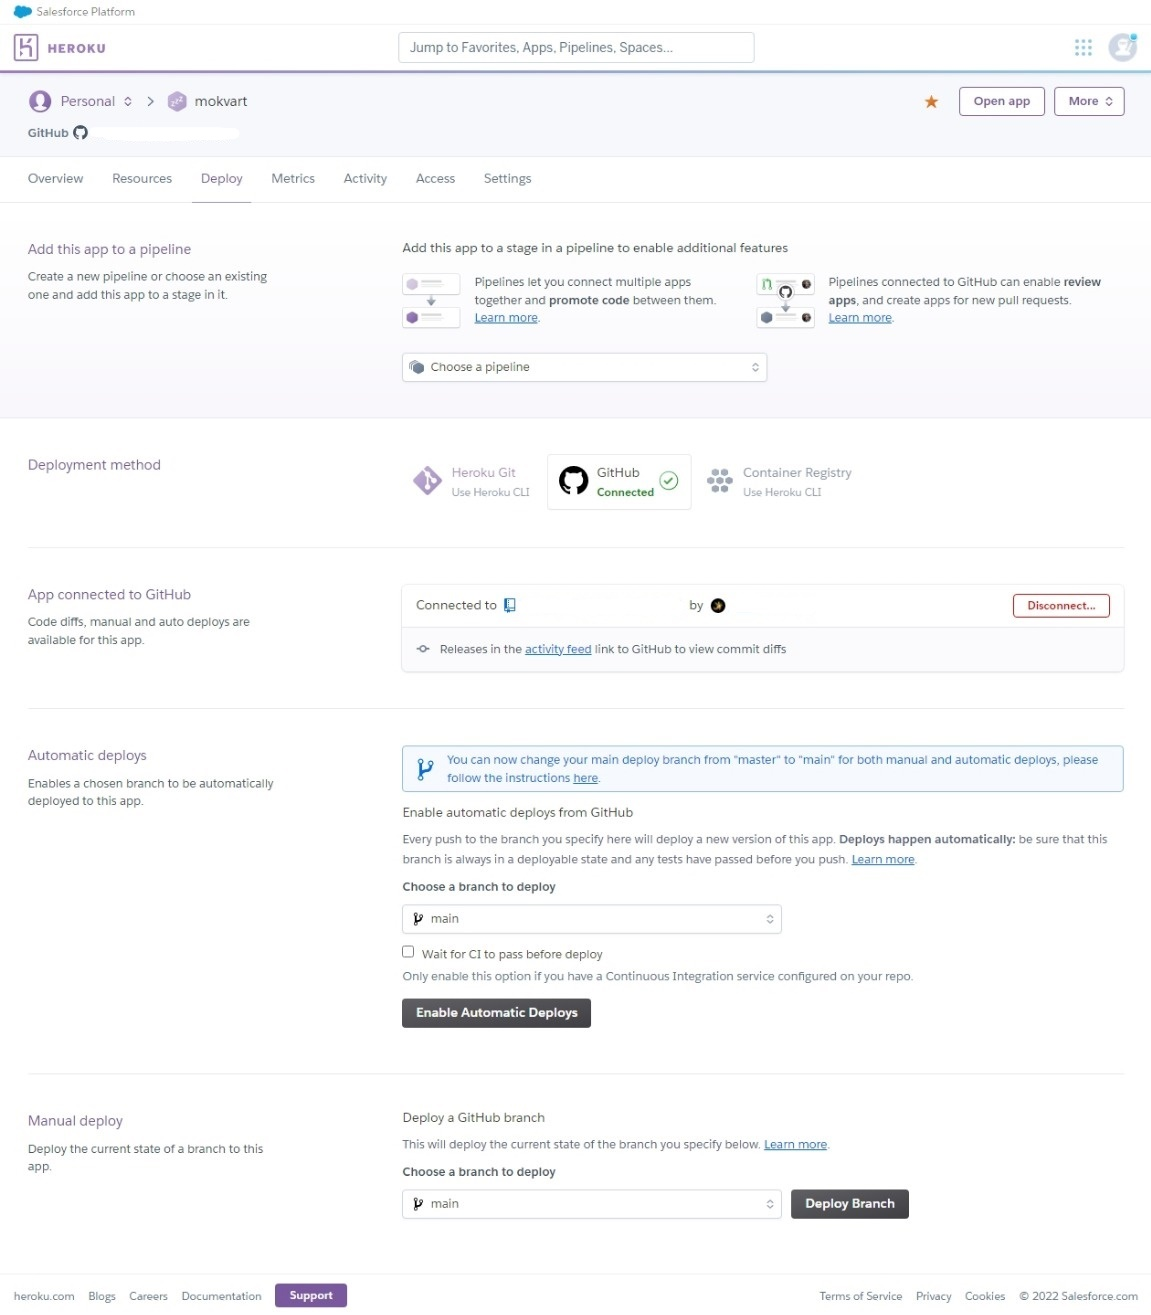
\includegraphics[width=\textwidth,keepaspectratio]{20 heroku screenshot.png}
					\caption{Prikaz aplikacije na poslužitelju Heroku}
				\end{figure}
				
				\begin{figure}[H]
					\centering
					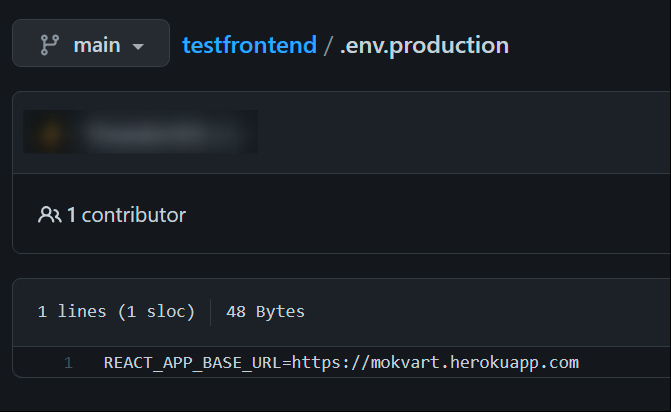
\includegraphics[width=\textwidth,keepaspectratio]{21 URL config.png}
					\caption{Povezivanje frontenda i backenda}
				\end{figure}
				
				\begin{figure}[H]
					\centering
					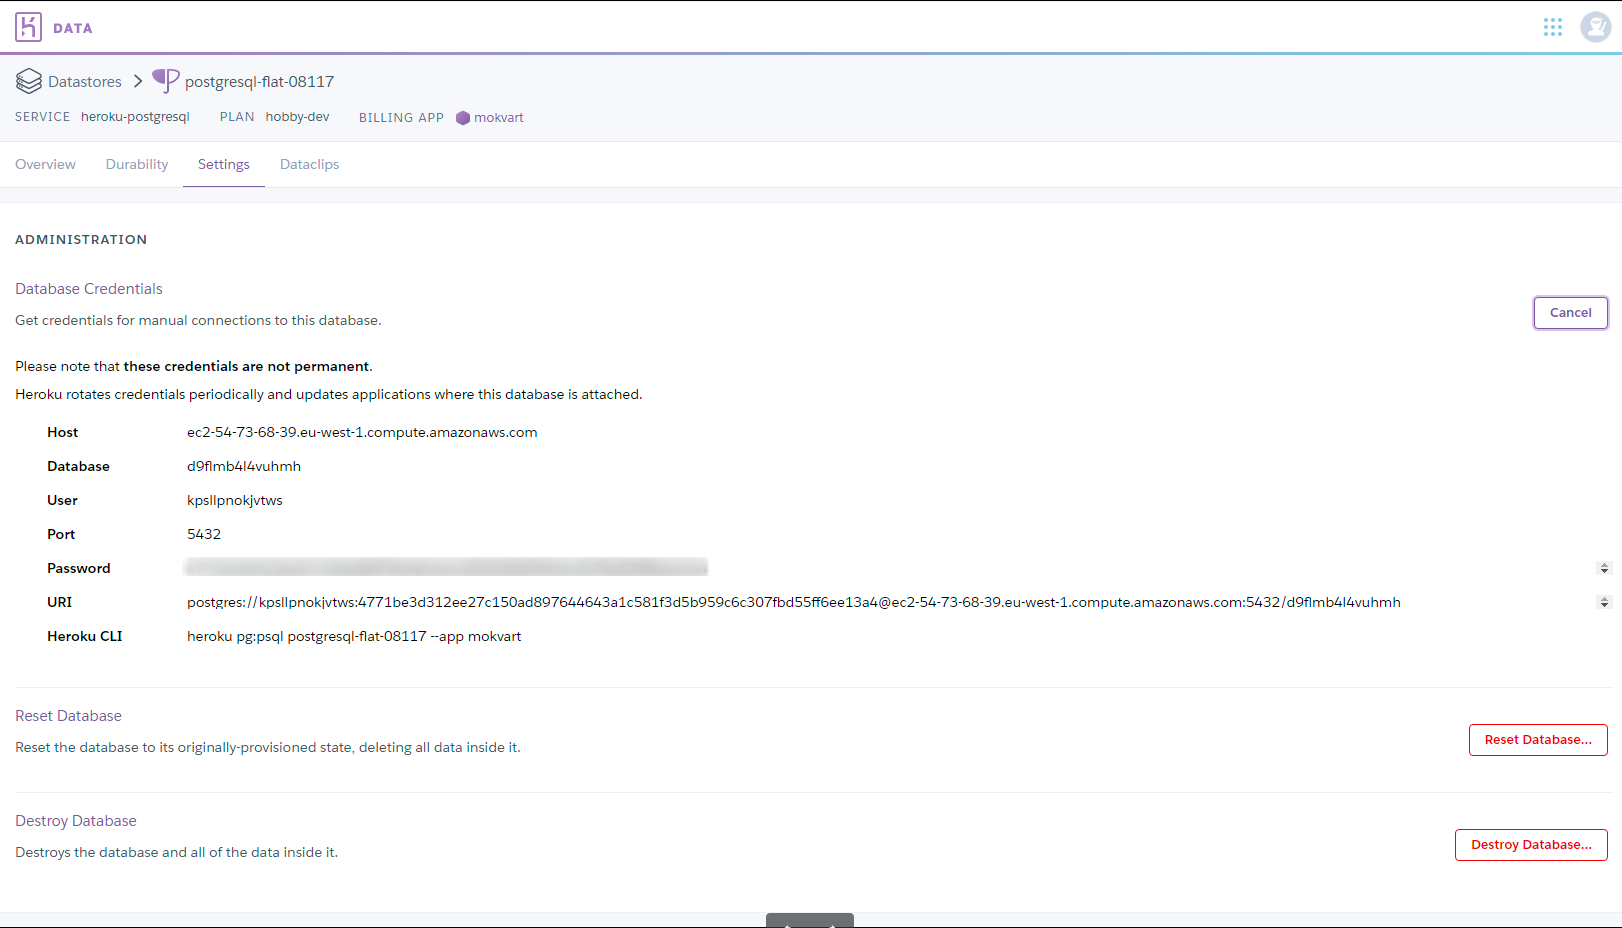
\includegraphics[width=\textwidth,keepaspectratio]{22 baza podaci.png}
					\caption{Podaci za pristup bazi}
				\end{figure}
				
				\begin{figure}[H]
					\centering
					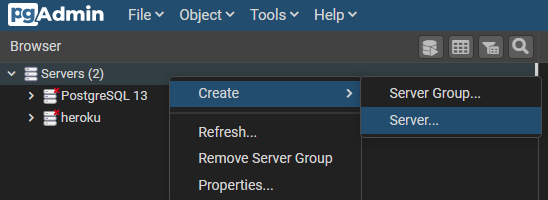
\includegraphics[width=\textwidth,keepaspectratio]{23 baza povezivanje.png}
					\caption{Pristup bazi lokalno u pgAdminu}
				\end{figure}

			\eject